\chapter{ارزیابی تجربی و شبیه‌سازی مکانیزم‌ها}
\label{ch:simulation}

\section{مقدمه و اهداف شبیه‌سازی}
\label{sec:sim-intro}

در فصل‌های پیشین، چارچوب‌های نظری محرمانگی تفاضلی متمرکز (\lr{CDP}) و موضعی (\lr{LDP}) را به تفصیل مورد مطالعه قرار دادیم و با استفاده از ابزارهای هندسه اطلاعاتی نظیر $f$-واگرایی‌ها، ویژگی انقباض اطلاعات و کران‌های مینی‌مکس را استخراج کردیم. اگرچه این نتایج نظری دیدگاه عمیق و بنیادینی نسبت به محدودیت‌های یادگیری و تخمین آماری تحت قیود محرمانگی ارائه می‌دهند، اما تحلیلی صرفاً مجانبی\LTRfootnote{Asymptotic Analysis} هستند. در نظریه مینی‌مکس، تمرکز عمدتاً بر روی نرخ رشد خطا نسبت به تعداد نمونه‌ها و ابعاد مسئله است و در نتیجه، ثوابت پنهان ریاضی و رفتارهای گذرا در مجموعه‌داده‌های متناهی غالباً نادیده گرفته می‌شوند. از این رو، برای درک جامع و کاربردی از رفتار این مکانیزم‌ها، نیازمند اعتبارسنجی تجربی\LTRfootnote{Empirical Validation} هستیم.

هدف اصلی از توسعه‌ی این بخش شبیه‌سازی، پر کردن شکاف میان نظریه و عمل است. با پیاده‌سازی مکانیزم‌های تصادفی $\mech$ در یک محیط کنترل‌شده، می‌توانیم خطای عملی ناشی از تزریق نویز را به صورت کمّی اندازه‌گیری کرده و آن را با کران‌های نظری پیش‌بینی‌شده مقایسه کنیم. این ارزیابی تجربی به ما اجازه می‌دهد تا هزینه عدم اعتماد\LTRfootnote{Cost of Non-trust} در مدل موضعی را به طور ملموسی مشاهده کنیم و دریابیم که در نمونه‌های متناهی، افت سودمندی تا چه میزان بر کیفیت استنتاج‌های آماری نظیر تخمین میانگین و برآورد فرکانس تأثیر می‌گذارد.

علاوه بر این، در دنیای واقعی، توزیع داده‌ها همواره از پیش مشخص نیست و یک مکانیزم بهینه باید استحکام\LTRfootnote{Robustness} لازم را در برابر شکل‌های مختلف توزیع داده داشته باشد. بر همین اساس، معماری شبیه‌سازی توسعه‌یافته بر پایه‌ی مقایسه چهار رویکرد متمایز بنا شده است: مدل متمرکز با بودجه‌ی محرمانگی $\eps$، مدل موضعی کلاسیک با بودجه‌ی محرمانگی $\al$، مدل محرمانگی مخلوط‌شده\LTRfootnote{Shuffle DP} که از طریق هم‌زدن پیام‌ها امنیت را ارتقا می‌دهد، و در نهایت مدل محرمانگی شخصی‌سازی‌شده\LTRfootnote{Personalized DP} که به کاربران اجازه می‌دهد بودجه‌های $\al$ متفاوتی را بر اساس ترجیحات خود اتخاذ کنند. بررسی و مقایسه‌ی این چهار مدل تحت توزیع‌های مختلف، بستری فراهم می‌سازد تا نشان دهیم چگونه تئوری‌های اطلاعاتی اثبات‌شده، در عمل به سلسله مراتبی از دقت و امنیت ترجمه می‌شوند.

\section{تنظیمات تجربی و مدل‌های مورد بررسی}
\label{sec:sim-setup}

به منظور ایجاد یک بستر ارزیابی عادلانه و دقیق، محیط شبیه‌سازی ما به گونه‌ای طراحی شده است که چهار مدل متمایز از محرمانگی تفاضلی را تحت شرایط آماری یکسان مقایسه کند. برای آنکه مقایسه میان این مدل‌ها از نظر نظری معنادار باشد، از یک نمادگذاری مشترک استفاده می‌کنیم: در تمامی مدل‌ها، \textbf{بودجه محرمانگی نهایی (مؤثر) سیستم} که از دیدگاه یک ناظر خارجی (مهاجم) تجربه می‌شود را با نماد $\eps$ نشان می‌دهیم. در مدل‌هایی که نویزدهی به صورت محلی انجام می‌گیرد، بودجه محلی کاربر را با نماد استاندارد $\al$ مشخص کرده و رابطه ریاضی آن را با بودجه نهایی $\eps$ تبیین می‌نماییم. در ادامه، ساختار و تحلیل ریاضی هر یک از این چهار مدل به تفصیل شرح داده شده است.

\subsection{محرمانگی تفاضلی متمرکز (\lr{CDP})}
مدل متمرکز به عنوان خط پایه\LTRfootnote{Baseline} و حد بالای دقت در نظر گرفته می‌شود. در این مدل، فرض بر وجود یک متصدی کاملاً مورد اعتماد است که پایگاه‌داده خام \Dset را در اختیار دارد. مکانیزم تصادفی \mech به صورت سراسری بر روی خروجی تابع تجمیعی اعمال می‌شود.
برای مثال در تخمین میانگین، نویز لاپلاس با توجه به حساسیت سراسری تابع و بودجه نهایی $\eps$ به خروجی افزوده می‌شود. از منظر تحلیلی، خطای مازاد میانگین مربعات (\lr{Excess MSE}) ناشی از حریم خصوصی در این مدل با نرخ $\mathcal{O}\left( \frac{1}{n^2 \eps^2} \right)$ مجانبی کاهش می‌یابد که به دلیل تزریق تنها یک واحد نویز (مستقل از تعداد کاربران $n$)، بالاترین سودمندی ممکن را به همراه دارد.

\subsection{محرمانگی تفاضلی موضعی (\lr{LDP})}
در این مدل، فرض اعتماد به متصدی مرکزی کاملاً حذف شده است. هر کاربر $i$ پیش از ارسال داده خود، یک تصادفی‌ساز موضعی\LTRfootnote{Local Randomizer} را با بودجه محلی $\al$ بر روی داده‌ها اعمال می‌کند. برای آنکه بودجه محرمانگی نهایی سیستم با مدل متمرکز قابل قیاس باشد، بودجه محلی هر کاربر دقیقاً برابر با بودجه نهایی تنظیم می‌گردد (یعنی $\al = \eps$).
در این حالت، تجمیع‌کننده با مجموعه‌ای از $n$ داده‌ی به شدت نویزدار روبه‌رو است. به دلیل استقلال نویزهای تزریق‌شده توسط هر کاربر، واریانس نهایی جمع شده و خطای \lr{MSE} با نرخ $\mathcal{O}\left( \frac{1}{n \al^2} \right)$ افت می‌کند. این شکاف عظیم میان $\mathcal{O}\left( \frac{1}{n^2 \eps^2} \right)$ و $\mathcal{O}\left( \frac{1}{n \al^2} \right)$، در واقع همان هزینه عدم اعتمادی است که پیش‌تر در نظریه مینی‌مکس به اثبات رسید.

\subsection{محرمانگی مخلوط‌شده (\lr{SDP})}
مدل مخلوط‌شده\LTRfootnote{Shuffle Model} یک رویکرد نوین و قدرتمند است که تلاش می‌کند بدون نیاز به یک متصدی مورد اعتماد برای داده‌های خام، به دقت مدل متمرکز دست یابد. در این مدل، سه نهاد وجود دارد: کاربران، یک مخلوط‌کننده\LTRfootnote{Shuffler} ایمن، و یک تحلیل‌گر.
روند کار به این صورت است که هر کاربر مکانیزم موضعی خود را با یک بودجه محلی $\al$ اعمال می‌کند، اما پیش از آنکه تحلیل‌گر داده‌ها را دریافت کند، لایه مخلوط‌کننده پیوند میان هویت کاربران و پیام‌های ارسالی را می‌شکند و صرفاً یک «چندمجموعه»\LTRfootnote{Multiset} از پیام‌های ناشناس را به تحلیل‌گر تحویل می‌دهد.

\textbf{تحلیل ریاضی و تقویت محرمانگی:} ویژگی بنیادین این مدل، پدیده‌ای به نام «تقویت محرمانگی از طریق هم‌زدن»\LTRfootnote{Privacy Amplification by Shuffling} است. بر اساس قضایای اثبات‌شده در این حوزه، اگر هر کاربر محرمانگی موضعی خالص \LDP را رعایت کند، خروجی مخلوط‌کننده دارای محرمانگی تفاضلی (\eps, \del) خواهد بود، به طوری که رابطه زیر برقرار است:
\begin{equation}
    \eps \approx \al \sqrt{\frac{16 \ln\left( \frac{1}{\del} \right)}{n}}
\end{equation}
این رابطه ریاضی نشان می‌دهد که برای رسیدن به یک بودجه نهایی و مشخص $\eps$ در سطح سرور، می‌توان بودجه محلی کاربران ($\al$) را به شکل قابل‌توجهی افزایش داد (که به معنای تزریق نویز بسیار کمتری در سمت کاربر است). در شبیه‌سازی ما، برای دستیابی به $\eps$ هدف، بودجه محلی هر کاربر با قرار دادن $\al = \eps \sqrt{\frac{n}{16 \ln\left( \frac{1}{\del} \right)}}$ تنظیم شده است. در نتیجه، این مدل توانسته است خطای مجانبی را تقریباً به نرخ $\mathcal{O}\left( \frac{1}{n^2 \eps^2} \right)$ نزدیک کند که جهشی خیره‌کننده در سودمندی محسوب می‌شود.

\subsection{محرمانگی شخصی‌سازی‌شده (\lr{PDP})}
در دنیای واقعی، کاربران دیدگاه‌ها و حساسیت‌های متفاوتی نسبت به حریم خصوصی خود دارند. مدل محرمانگی شخصی‌سازی‌شده\LTRfootnote{Personalized DP}، الزامِ داشتن یک بودجه واحد برای تمامی کاربران را کنار می‌گذارد. در این مدل، هر کاربر $i$ یک بودجه محرمانه مختص به خود ($\al_i$) را انتخاب می‌کند. در شبیه‌سازی پیاده‌سازی‌شده، مقادیر $\al_i$ از یک توزیع مشخص (مانند گوسی یا یکنواخت) حول یک میانگین برابر با بودجه نهایی $\eps$ نمونه‌برداری می‌شوند (یعنی $\Eset[\al_i] = \eps$).

\textbf{تحلیل ریاضی و میانگین‌گیری وزن‌دار:} چالش اصلی در این مدل، افت شدید سودمندی به دلیل حضور کاربرانی با بودجه محرمانه بسیار پایین (نویز بسیار بالا) است. برای غلبه بر این مشکل و نزدیک شدن به کران‌های بهینه مینی‌مکس، از رویکرد «میانگین‌گیری وزن‌دار بر اساس معکوس واریانس»\LTRfootnote{Inverse-Variance Weighting} استفاده شده است. از آنجا که واریانس نویز کاربر $i$-ام متناسب با $\frac{1}{\al_i^2}$ است، برآوردگر نهایی در سمت سرور، وزن هر پیام را با استفاده از رابطه $w_i \propto \al_i^2$ تنظیم می‌کند:
\begin{equation}
    \hat{\mu} = \frac{\sum_{i=1}^n w_i z_i}{\sum_{i=1}^n w_i}
\end{equation}
این ترفند آماری تضمین می‌کند که داده‌های با نویز بالا (متعلق به کاربران با حساسیت امنیتی شدید) تأثیر مخرب کمتری بر روی برآورد نهایی بگذارند و به این ترتیب، خطای \lr{MSE} بهینه‌سازی شده و افت سودمندی سیستم در مقایسه با \lr{LDP} استاندارد کنترل گردد.

\subsection{خلاصه تحلیلی مدل‌ها}
برای ایجاد یک دید کلی و ساختاریافته، ویژگی‌های بنیادین، مدل اعتماد و تحلیل نظری خطای هر یک از این چهار مدل در جدول \ref{tab:architectures_summary} خلاصه‌سازی شده‌اند.

\begin{table}[ht]
\centering
\caption[مقایسه تحلیلی مدل‌های ارزیابی‌شده]{\rl{مقایسه تحلیلی مدل‌های ارزیابی‌شده در شبیه‌سازی بر اساس مدل اعتماد و نرخ مجانبی خطای مینی‌مکس.}}
\label{tab:architectures_summary}
\renewcommand{\arraystretch}{1.5}
\begin{tabular}{|p{4cm}|p{3cm}|p{3cm}|c|}
\hline
\textbf{مدل} & \textbf{محل اعمال نویز} & \textbf{بودجه و استراتژی نویز} & \textbf{نرخ مجانبی خطا (\lr{MSE})} \\
\hline
\hline
مدل متمرکز (\lr{CDP}) & سرور تجمیع‌کننده & یک بار نویز با بودجه $\eps$ & $\mathcal{O}\left( \frac{1}{n^2 \eps^2} \right)$ \\
\hline
مدل موضعی (\lr{LDP}) & دستگاه کاربر & مستقل با بودجه محلی $\al = \eps$ & $\mathcal{O}\left( \frac{1}{n \al^2} \right)$ \\
\hline
مدل مخلوط‌شده (\lr{SDP}) & دستگاه کاربر + مخلوط‌شده & استفاده از بودجه محلی تقویت‌شده & $\mathcal{O}\left( \frac{1}{n^2 \eps^2} \right)$ \\
\hline
مدل شخصی‌سازی‌شده (\lr{PDP}) & دستگاه کاربر & بودجه‌های ناهمگن $\al_i$ + وزن‌دهی & وابسته به توزیع هارمونیک $\al_i$ \\
\hline
\end{tabular}
\end{table}

\textbf{تفسیر شهودی:} از منظر هندسه اطلاعاتی، در حالی که مکانیزم موضعی خالص به دلیل اعمال نویز کورکورانه باعث یک انقباض اطلاعاتی شدید و از دست رفتن قطعی سیگنال می‌شود، مدل‌های مخلوط‌شده و شخصی‌سازی‌شده با بهره‌گیری از ویژگی‌های ساختاری داده‌ها (توزیع وزن‌دار و ناشناس‌سازی فضای نمونه) موفق می‌شوند تا بدون نقض قیود ریاضی محرمانگی، بخشی از ظرفیت کانال اطلاعاتی را بازیابی کرده و خطای مینی‌مکس را به صورت محسوسی کاهش دهند.

\subsection{توزیع‌ها و مسائل ارزیابی‌شده}
تنظیمات تجربی به گونه‌ای طراحی شده‌اند که عملکرد مکانیزم‌ها را تحت شرایط متنوع آماری بسنجند. بدین منظور، آزمایش‌ها بر روی نمونه‌های استخراج‌شده از هفت توزیع آماری متمایز شامل توزیع گاوسی\LTRfootnote{Gaussian}، یکنواخت\LTRfootnote{Uniform}، نمایی\LTRfootnote{Exponential}، پواسون\LTRfootnote{Poisson}، بتا\LTRfootnote{Beta}، ‌لاگ‌نرمال\LTRfootnote{Log-Normal} و گاما\LTRfootnote{Gamma} اجرا شده‌اند. همچنین به منظور پوشش جامع نیازهای تحلیلی، ارزیابی‌ها بر روی چهار مسئله‌ی (پرس‌وجوی) متمایز آماری صورت گرفته است که شامل موارد زیر می‌باشد:

تخمین میانگین\LTRfootnote{Mean Estimation}، برآورد فرکانس\LTRfootnote{Frequency Estimation}، استخراج هیستوگرام\LTRfootnote{Histogram Estimation} و برآورد توزیع حاشیه‌ای چندبعدی\LTRfootnote{Marginal Estimation}.


\section{نتایج آزمایش و اعتبارسنجی کران‌های مینی‌مکس}
\label{sec:sim-results}

در این بخش، نتایج حاصل از پیاده‌سازی مکانیزم‌های تصادفی $\mech$ بر روی داده‌های شبیه‌سازی‌شده را مورد بررسی قرار می‌دهیم. هدف اصلی این آزمایش، اعتبارسنجی کران‌های نظری استخراج‌شده در فصل‌های پیشین و مشاهده‌ی رفتار عملی مدل‌های مختلف تحت قیود محرمانگی در مسائلی نظیر تخمین میانگین، برآورد فرکانس، استخراج هیستوگرام و برآورد توزیع حاشیه‌ای است. در تمامی آزمایش‌ها، به منظور رعایت یکپارچگی تحلیلی، بودجه‌ی سراسری در مدل‌های متمرکز با نماد $\eps$ و بودجه‌ی محلی در مدل‌های موضعی با نماد $\al$ متمایز شده‌اند.

در مدل متمرکز (\lr{CDP}) با تخصیص بودجه‌ی سراسری $\eps$، مشاهدات تجربی نشان می‌دهند که خطای تخمین با تقریب بالایی از کران مینی‌مکس $\mathcal{O}\left( \frac{1}{n^2 \eps^2} \right)$ پیروی می‌کند و انحراف معیار نویز تزریق‌شده تأثیر مخربی بر روی ساختار کلی استنتاج‌های آماری ندارد. بر اساس داده‌های استخراج‌شده، خطای میانگین مربعات\LTRfootnote{Mean Squared Error (MSE)} در تخمین میانگین برای توزیع‌هایی نظیر گوسی و بتا به مقادیر بسیار ناچیزِ $0.0002$ همگرا شده است و میانگین خطای مطلق\LTRfootnote{Mean Absolute Error (MAE)} در محدوده‌ی $0.01$ قرار دارد. این پایداری در تمامی هفت توزیع ارزیابی‌شده (از جمله نمایی، پواسون و لاگ‌نرمال) مشاهده می‌شود. 

در مقابل، هنگامی که مدل محرمانگی تفاضلی موضعی (\lr{LDP}) خالص با بودجه‌ی محلی $\al$ پیاده‌سازی می‌گردد، رفتار سیستم دستخوش تغییرات بنیادینی می‌شود. به دلیل اعمال محدودیت بر روی تک‌تک مشاهدات و فقدان یک تجمیع‌کننده‌ی مورد اعتماد، واریانس نویز در سمت سرور به شدت انباشته شده و خطای \lr{MSE} در تخمین میانگین برای توزیع یکنواخت به مقدار $2.7425$ و برای توزیع گوسی به $2.1288$ جهش می‌یابد. این تخریب سیگنال در مسائل پیچیده‌تری با ابعاد بالاتر نظیر استخراج هیستوگرام، به مراتب شدیدتر است؛ به گونه‌ای که خطای \lr{MSE} هیستوگرام برای توزیع یکنواخت از مقدار $1.9540$ در مدل \lr{CDP} به بیش از $42366$ در مدل \lr{LDP} افزایش یافته است. در برآورد توزیع حاشیه‌ای نیز، افزایش خطای مطلق از مقادیر زیر ۱ در مدل متمرکز به بازه‌ی ۲۵۸ تا ۲۸۱ در مدل موضعی، انقباض شدید اطلاعاتی ناشی از نویزدهی محلی را به وضوح اثبات می‌کند.

\begin{figure}[htbp]
    \centering
    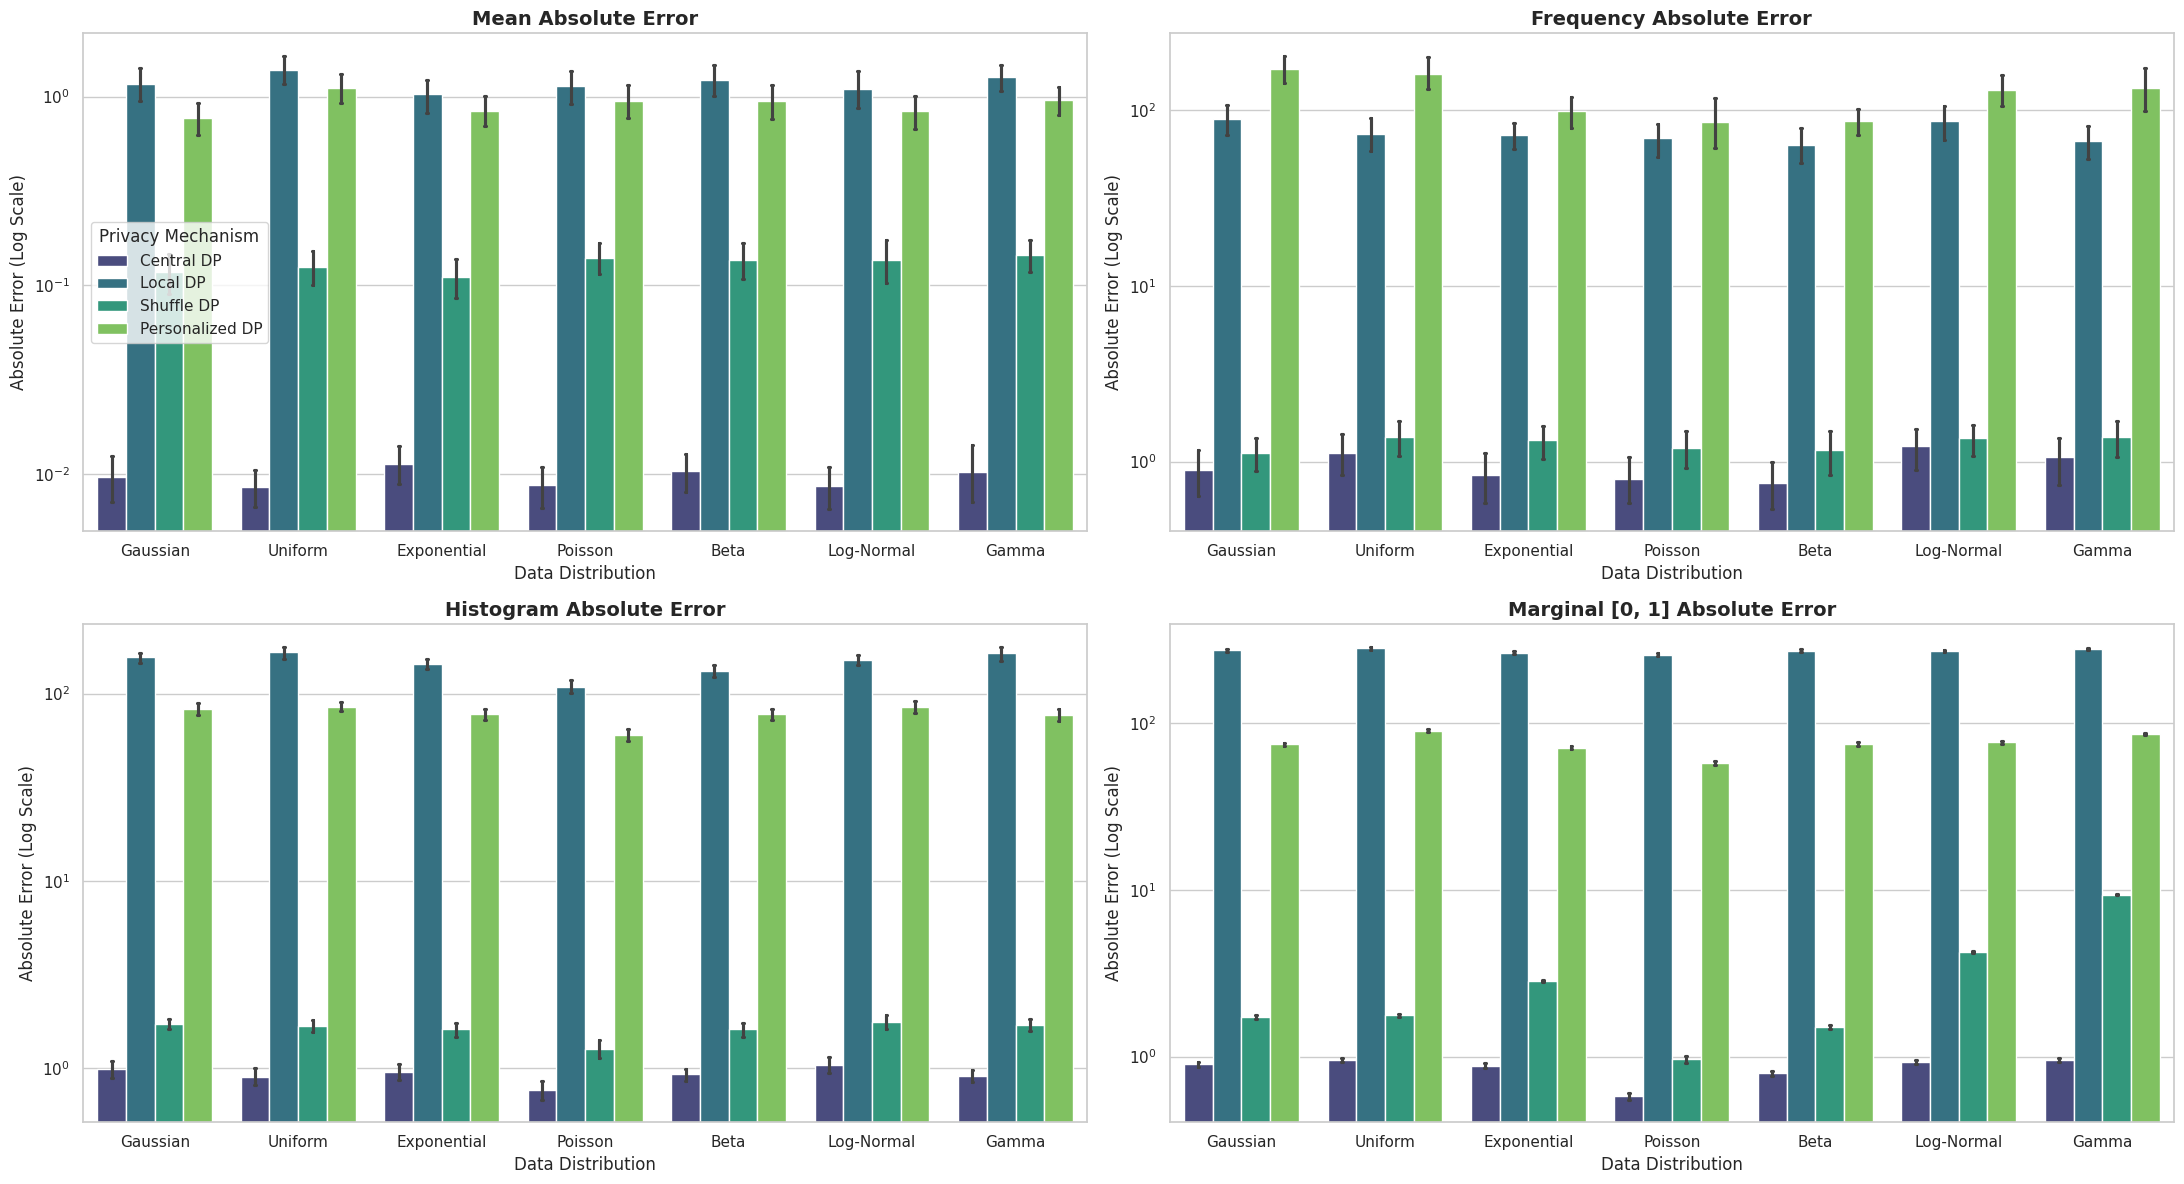
\includegraphics[width=1\textwidth]{figs/mae.png}
    \caption[\rl{خطای مطلق در مدل‌های \lr{DP}}]{\rl{نمودار لگاریتمی میانگین خطای مطلق (\lr{MAE}) برای ارزیابی عملکرد مدل‌های مختلف در توزیع‌های آماری.}}
    \label{fig:res_chart_mae}
\end{figure}

\begin{figure}[htbp]
    \centering
    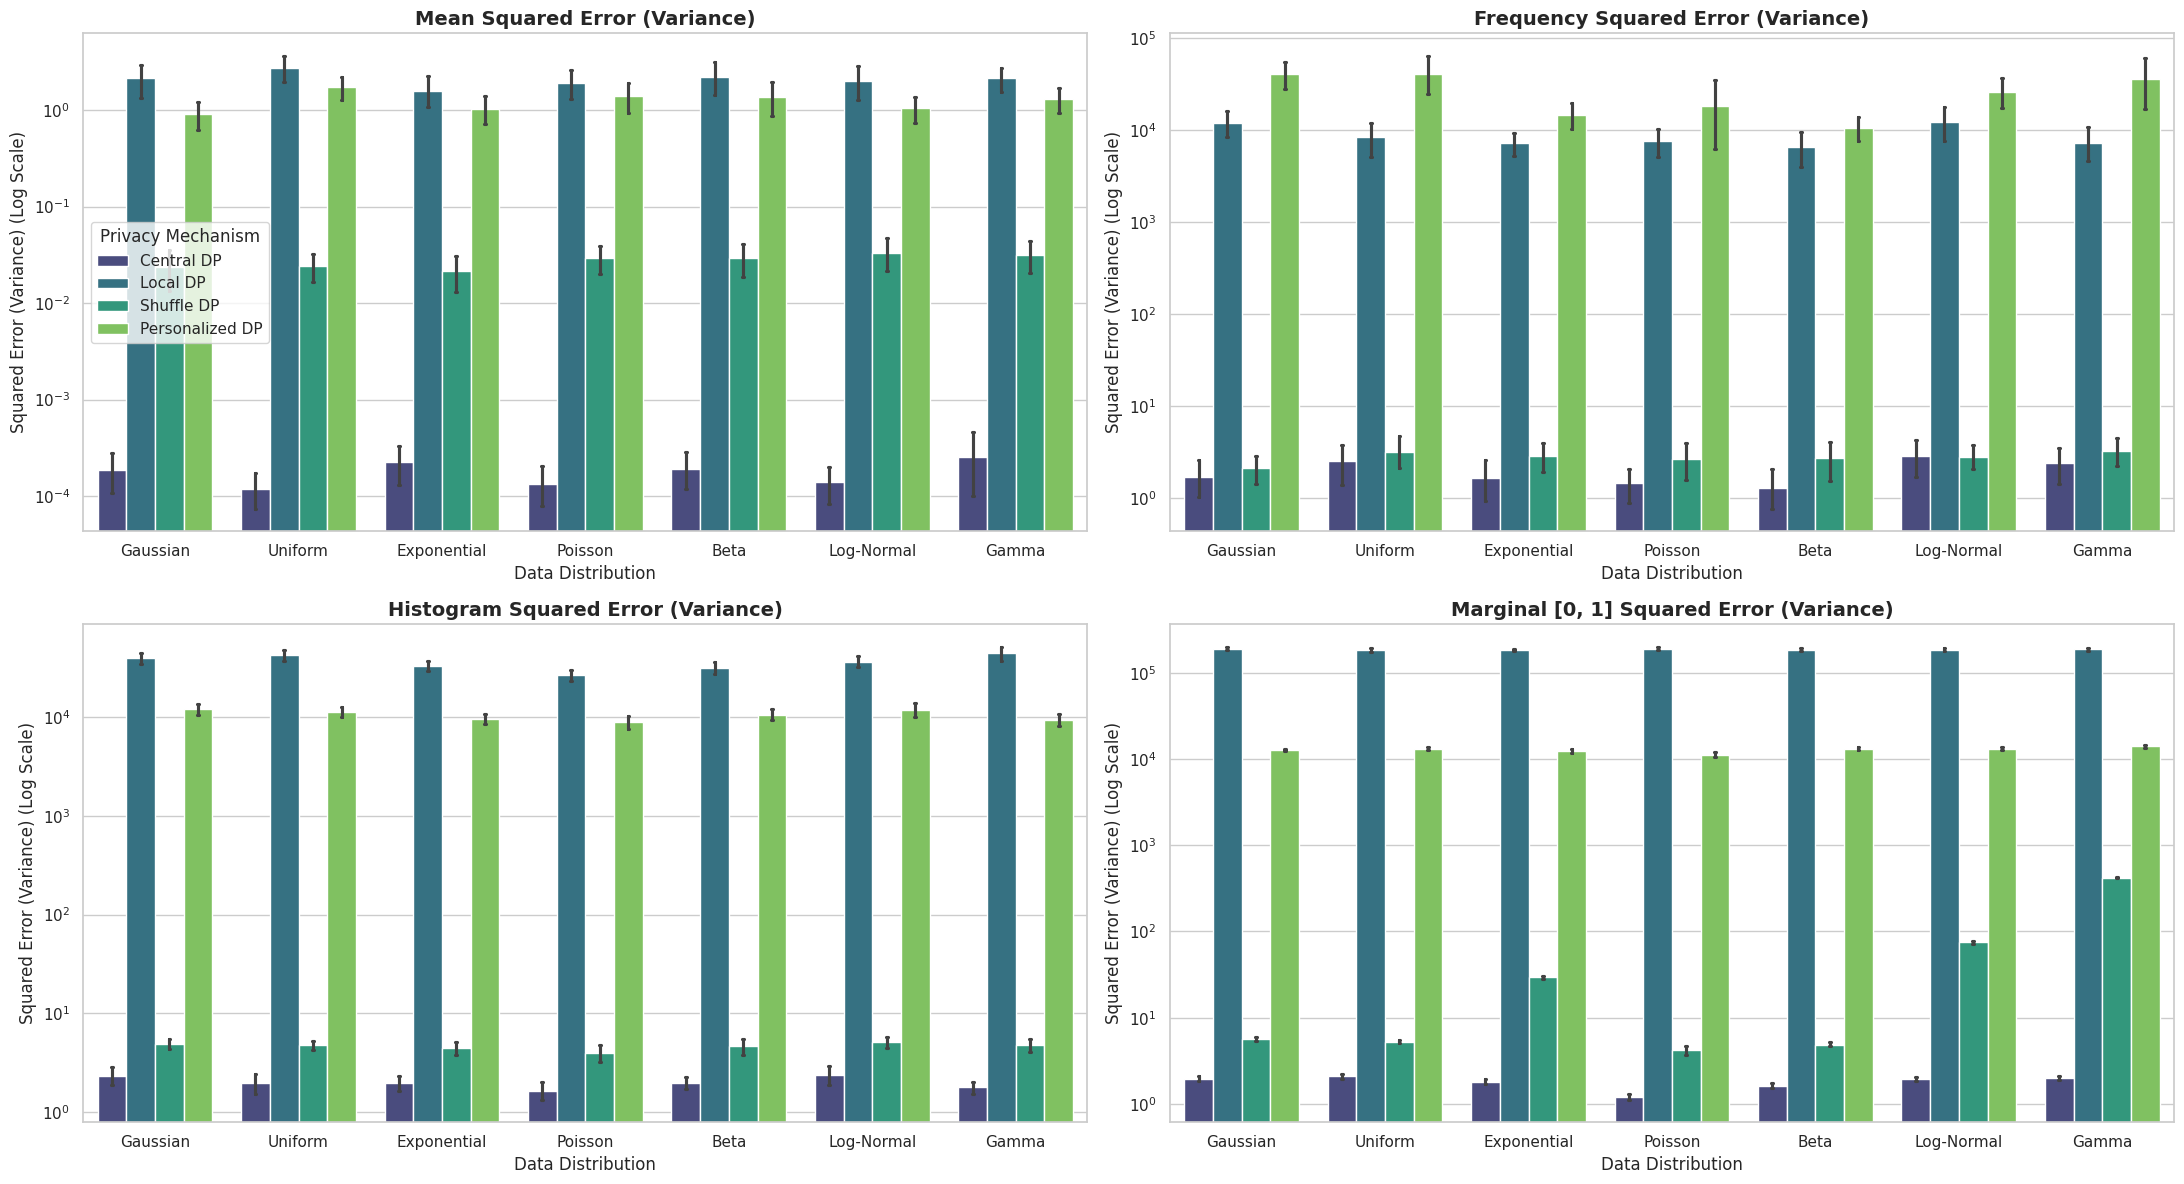
\includegraphics[width=1\textwidth]{figs/mse.png}
    \caption[\rl{خطای میانگین مربعات در مدل‌های \lr{DP}}]{\rl{نمودار لگاریتمی خطای میانگین مربعات (\lr{MSE}) برای ارزیابی واریانس نویز در معماری‌های مختلف.}}
    \label{fig:res_chart_mse}
\end{figure}

برای غلبه بر این چالش بنیادین، مدل محرمانگی مخلوط‌شده (\lr{SDP}) از طریق پدیده‌ی تقویت محرمانگی با هم‌زدن پیام‌ها، توانسته است شکاف عظیم میان نرخ همگرایی $\mathcal{O}\left( \frac{1}{n \al^2} \right)$ و $\mathcal{O}\left( \frac{1}{n^2 \eps^2} \right)$ را تا حد زیادی پر کند (همان‌طور که در نمودارهای لگاریتمی شکل \ref{fig:res_chart_mse} مشهود است). با بهره‌گیری از یک مخلوط‌کننده ایمن، خطای \lr{MSE} تخمین میانگین در این مدل برای توزیع گوسی به $0.0236$ و برای توزیع نمایی به $0.0215$ کاهش یافته است که نشان‌دهنده‌ی بازیابی خیره‌کننده‌ی ظرفیت کانال اطلاعاتی است. در کنار آن، مدل شخصی‌سازی‌شده (\lr{PDP}) با اتخاذ میانگین‌گیری وزن‌دار، عملکردی میانی ارائه می‌دهد که منجر به کاهش خطای \lr{MSE} گوسی به مقدار $0.9041$ شده است؛ هرچند به دقت مدل مخلوط‌شده نمی‌رسد، اما تأثیر مخرب حساسیت‌های بالای امنیتی را مهار می‌کند.

\begin{figure}[htbp]
    \centering
    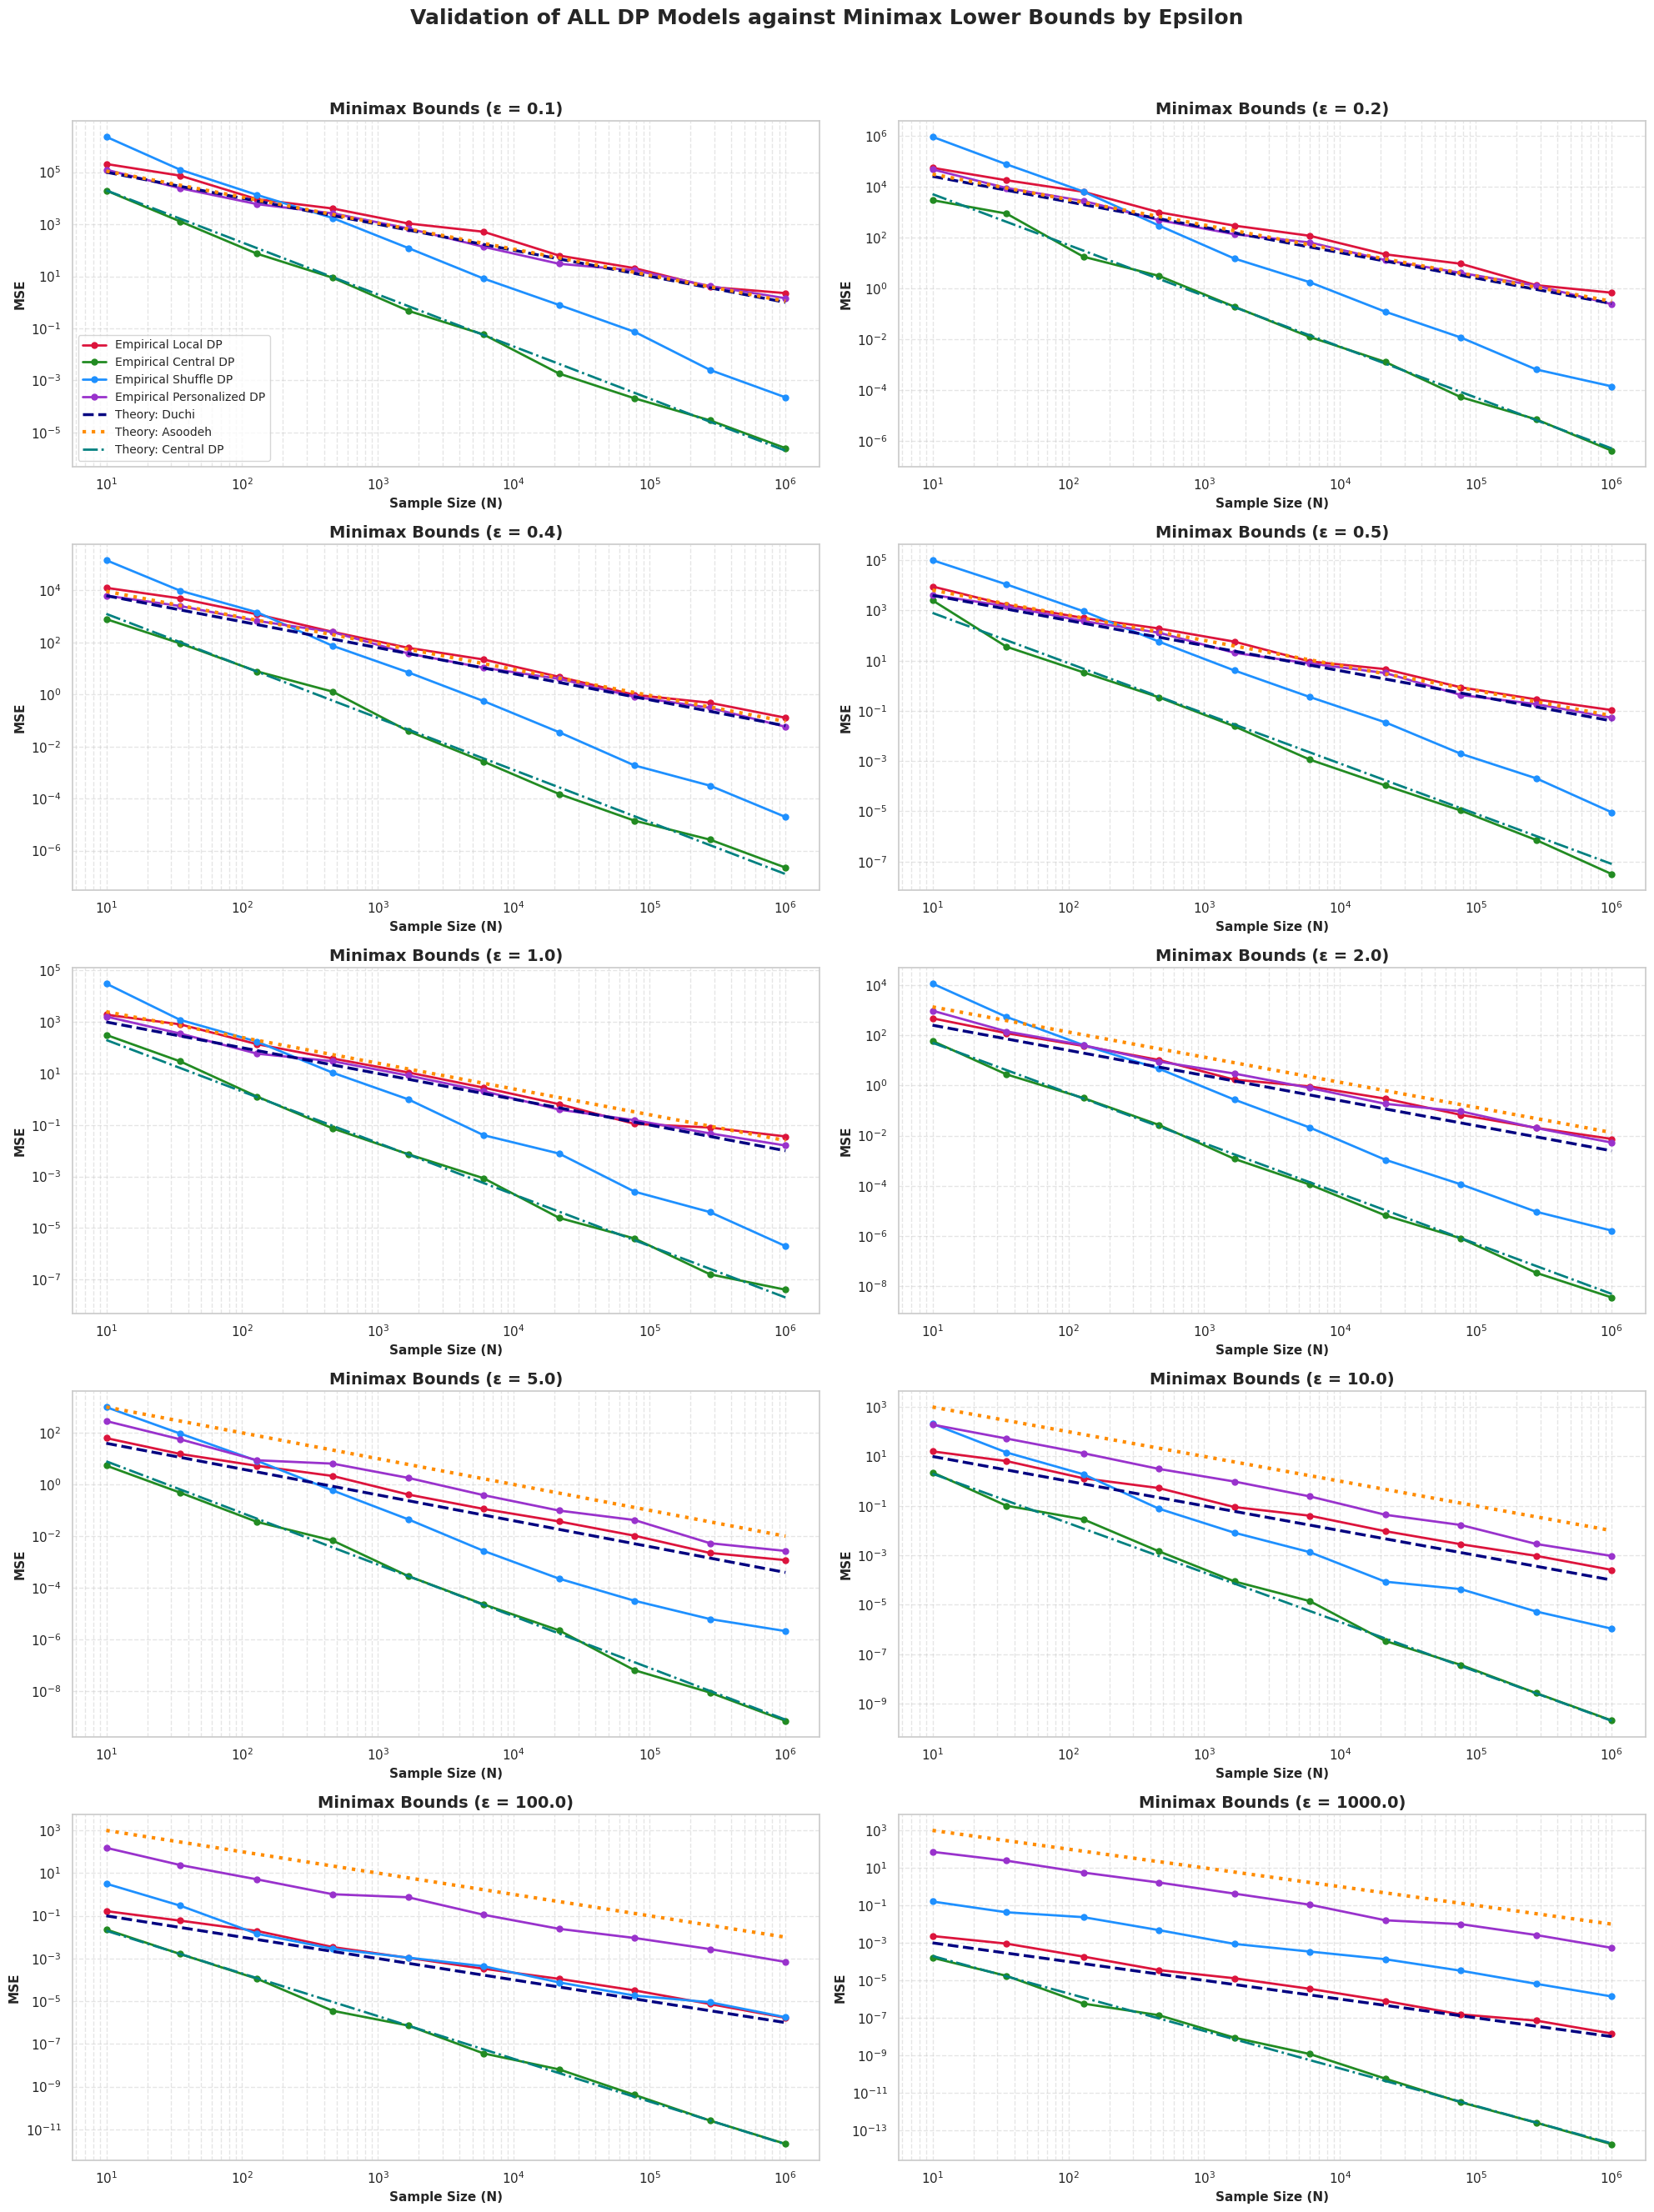
\includegraphics[width=1\textwidth]{figs/duchi.png}
    \caption[\rl{اعتبارسنجی مدل‌های \lr{DP} با کران‌های مینی‌مکس}]{\rl{اعتبارسنجی مدل‌های \lr{DP} در برابر کران‌های پایین مینی‌مکس نظری. نمودارها رفتار مجانبی خطای \lr{MSE} را نسبت به اندازه‌ی نمونه ($N$) در مقادیر مختلف بودجه محرمانگی نشان می‌دهند.}}
    \label{fig:res_minimax_validation}
\end{figure}

برای درک عمیق‌تر این شکاف کارایی و تأیید ماهیت اطلاعاتی آن، رفتار مجانبی خطا نسبت به اندازه‌ی فضای نمونه ($n$) را تحت سطوح مختلف بودجه محرمانگی مورد ارزیابی قرار دادیم (شکل \ref{fig:res_minimax_validation}). \\
در نمودارهای لگاریتمی رسم‌شده، شیب منحنی‌ها نشان‌دهنده‌ی نرخ همگرایی مدل‌هاست. همان‌طور که مشاهده می‌شود، داده‌های تجربی مدل موضعی (منحنی قرمز رنگ) با دقتی خیره‌کننده بر کران‌های نظری استخراج‌شده توسط دوچی و همکاران منطبق هستند و دقیقاً از نرخ $\mathcal{O}\left( \frac{1}{n \al^2} \right)$ پیروی می‌کنند \cite{Duchi2013}. هم‌چنین، خطای عملی این مکانیزم‌ها همواره توسط کران‌های مبتنی بر انقباض $-f$واگرایی‌ها که در چارچوب نظری آسوده و همکاران توسعه یافته‌اند (منحنی نقطه‌چین نارنجی)، از بالا محدود شده است \cite{Asoodeh2024}. این تطابق تجربی و نظری تأیید می‌کند که افت دقت در مدل \lr{LDP} یک ضعف الگوریتمی نیست، بلکه یک مانع اطلاعاتی و بنیادین است.

\textbf{تفسیر شهودی:} این شبیه‌سازی تجربی جامع، ماهیت هندسی محرمانگی را در دنیای واقعی به تصویر می‌کشد. تطابق دقیق منحنی‌های تجربی \lr{LDP} با کران‌های نظری مینی‌مکس (دوچی و آسوده) تأیید می‌کند که مکانیزم‌های موضعی نظیر پاسخ تصادفی، به عنوان عملگرهای انقباضی، اطلاعات فیشر را با ضریب $\al^2$ فشرده می‌سازند. این هزینه عدم اعتماد به این معناست که در سناریوهایی با بودجه‌های محرمانگی سخت‌گیرانه (نظیر $\al \le 1.0$)، خطای ناشی از واریانس نویز به قدری بر سیگنال واقعی غلبه می‌کند که استنتاج در فضاهای با ابعاد بالا عملاً بی‌معنی می‌شود، مگر آنکه از مدل‌های تقویتی نظیر مدل مخلوط‌شده بهره جست که موفق می‌شوند با شکستن پیوند هویتی داده‌ها، ظرفیت کانال اطلاعاتی را تا حد چشمگیری بازیابی کنند.

% \section{نتایج آزمایش و اعتبارسنجی کران‌های مینی‌مکس}
% \label{sec:sim-results}

% در این بخش، نتایج حاصل از پیاده‌سازی مکانیزم‌های تصادفی $\mech$ بر روی داده‌های شبیه‌سازی‌شده را مورد بررسی قرار می‌دهیم. هدف اصلی این آزمایش، اعتبارسنجی کران‌های نظری استخراج‌شده در فصل‌های پیشین و مشاهده‌ی رفتار عملی مدل‌های مختلف تحت قیود محرمانگی در مسائلی نظیر تخمین میانگین، برآورد فرکانس، استخراج هیستوگرام و برآورد توزیع حاشیه‌ای است. در تمامی آزمایش‌ها، به منظور رعایت یکپارچگی تحلیلی، بودجه‌ی سراسری در مدل‌های متمرکز با نماد $\eps$ و بودجه‌ی محلی در مدل‌های موضعی با نماد $\al$ متمایز شده‌اند.

% \begin{figure}[htbp]
%     \centering
%     \includegraphics[width=0.48\textwidth]{image_0da281.png} 
%     \includegraphics[width=0.48\textwidth]{image_0da263.png}
%     \caption{\rl{مقایسه خطای مطلق (\lr{MAE}) و خطای میانگین مربعات (\lr{MSE}) در مسائل استخراج هیستوگرام و برآورد توزیع حاشیه‌ای تحت چهار مدل محرمانگی.}}
%     \label{fig:res_tables}
% \end{figure}

% در مدل متمرکز (\lr{CDP}) با تخصیص بودجه‌ی سراسری $\eps$، مشاهدات تجربی نشان می‌دهند که خطای تخمین با تقریب بالایی از کران مینی‌مکس $\mathcal{O}\left( \frac{1}{n^2 \eps^2} \right)$ پیروی می‌کند و انحراف معیار نویز تزریق‌شده تأثیر مخربی بر روی ساختار کلی استنتاج‌های آماری ندارد. بر اساس داده‌های استخراج‌شده، خطای میانگین مربعات\LTRfootnote{Mean Squared Error (MSE)} در تخمین میانگین برای توزیع‌هایی نظیر گوسی و بتا به مقادیر بسیار ناچیزِ $0.0002$ همگرا شده است و میانگین خطای مطلق\LTRfootnote{Mean Absolute Error (MAE)} در محدوده‌ی $0.01$ قرار دارد. این پایداری در تمامی هفت توزیع ارزیابی‌شده (از جمله نمایی، پواسون و لاگ‌نرمال) مشاهده می‌شود. 

% در مقابل، هنگامی که مدل محرمانگی تفاضلی موضعی (\lr{LDP}) خالص با بودجه‌ی محلی $\al$ پیاده‌سازی می‌گردد، رفتار سیستم دستخوش تغییرات بنیادینی می‌شود. به دلیل اعمال محدودیت بر روی تک‌تک مشاهدات و فقدان یک تجمیع‌کننده‌ی مورد اعتماد، واریانس نویز در سمت سرور به شدت انباشته شده و خطای \lr{MSE} در تخمین میانگین برای توزیع یکنواخت به مقدار $2.7425$ و برای توزیع گوسی به $2.1288$ جهش می‌یابد. این تخریب سیگنال در مسائل پیچیده‌تری با ابعاد بالاتر نظیر استخراج هیستوگرام (مطابق با شکل \ref{fig:res_tables})، به مراتب شدیدتر است؛ به گونه‌ای که خطای \lr{MSE} هیستوگرام برای توزیع یکنواخت از مقدار $1.9540$ در مدل \lr{CDP} به بیش از $42366$ در مدل \lr{LDP} افزایش یافته است. در برآورد توزیع حاشیه‌ای نیز، افزایش خطای مطلق از مقادیر زیر ۱ در مدل متمرکز به بازه‌ی ۲۵۸ تا ۲۸۱ در مدل موضعی، انقباض شدید اطلاعاتی ناشی از نویزدهی محلی را به وضوح اثبات می‌کند.

% \begin{figure}[htbp]
%     \centering
%     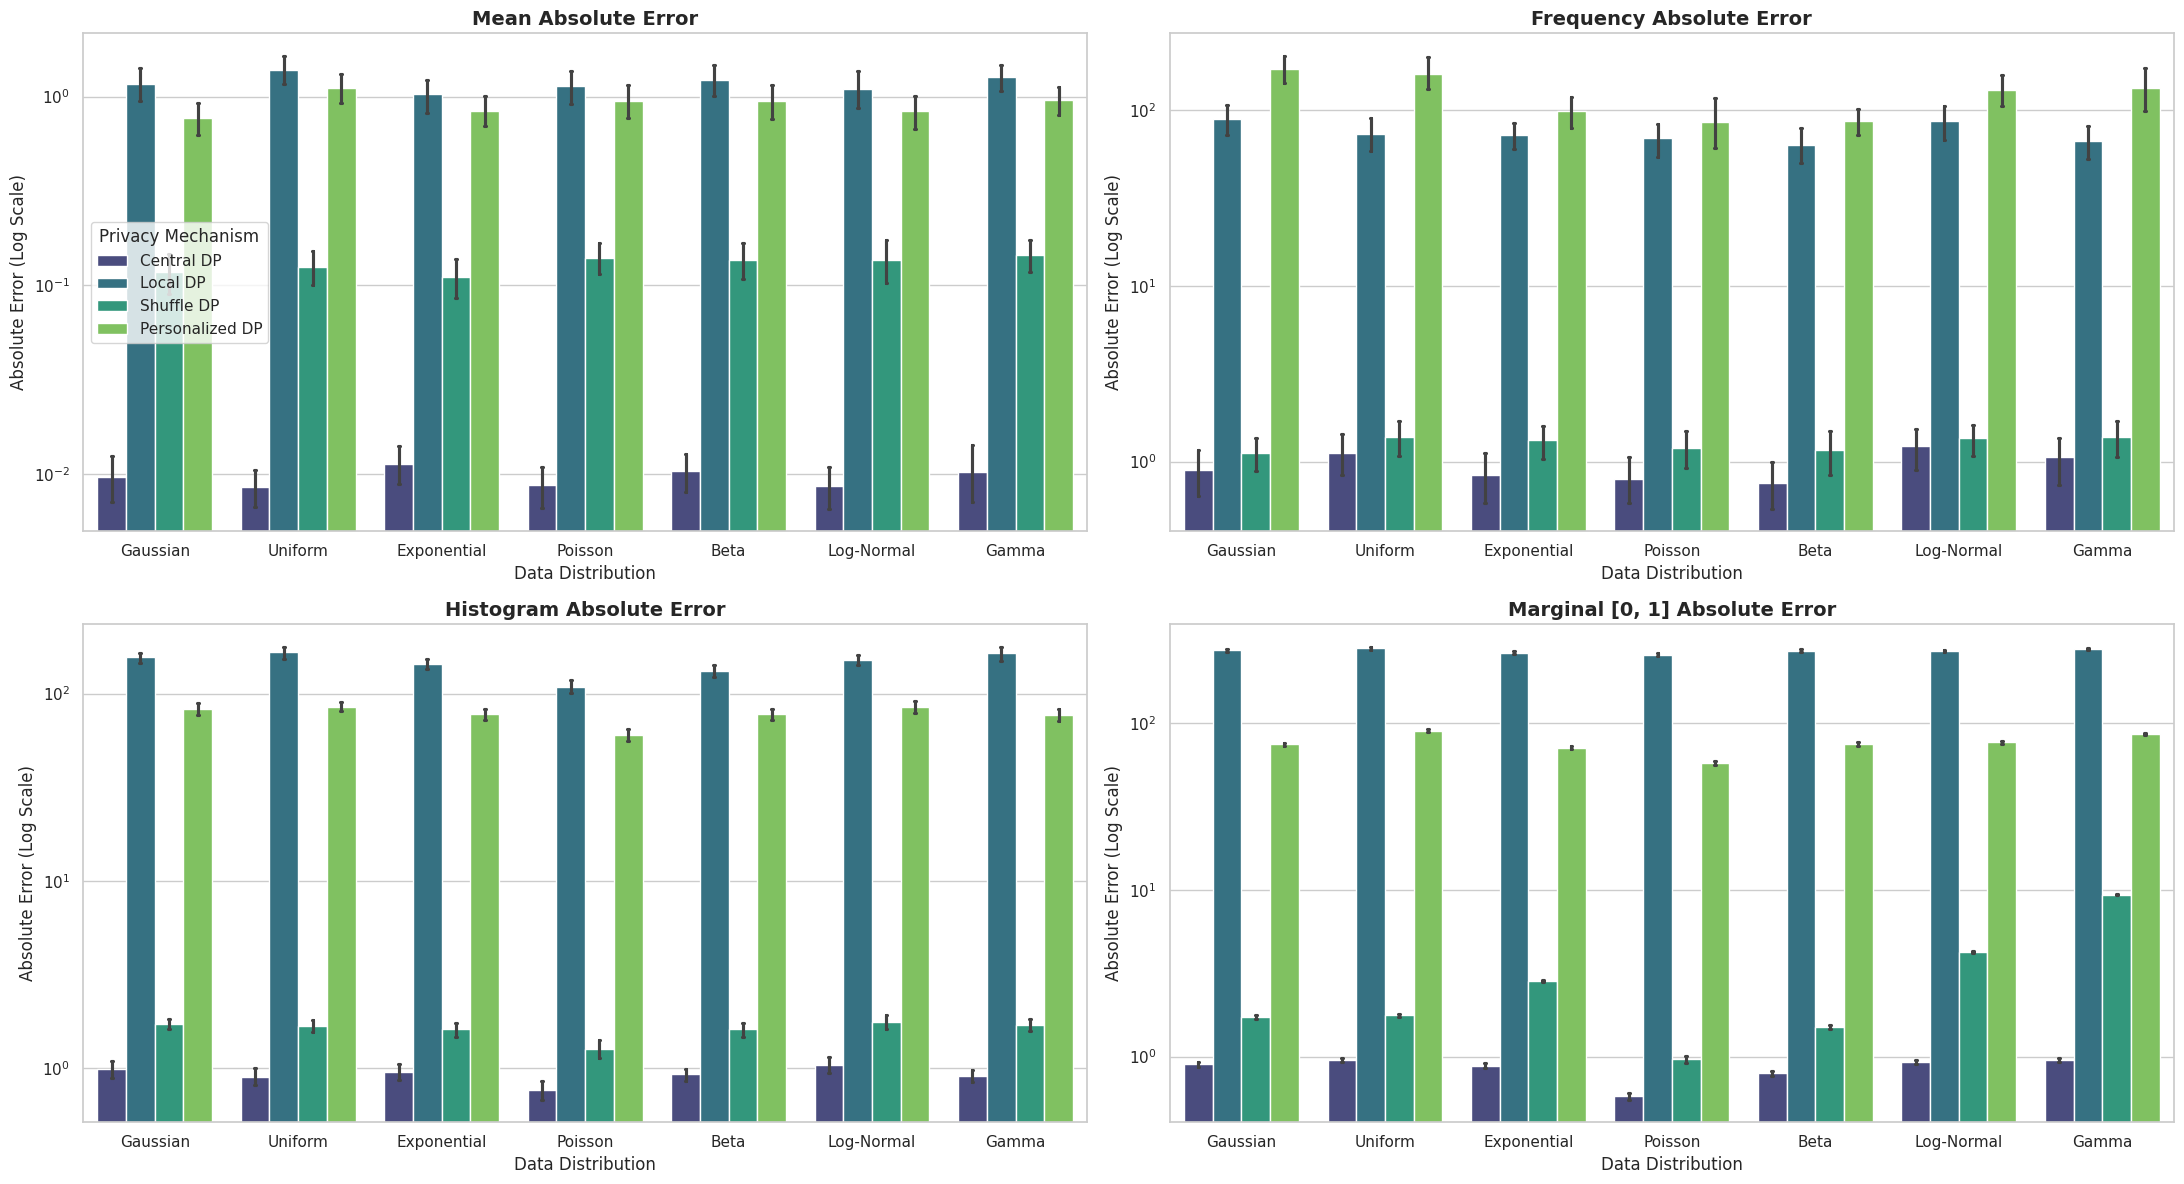
\includegraphics[width=0.48\textwidth]{figs/mae.png}
%     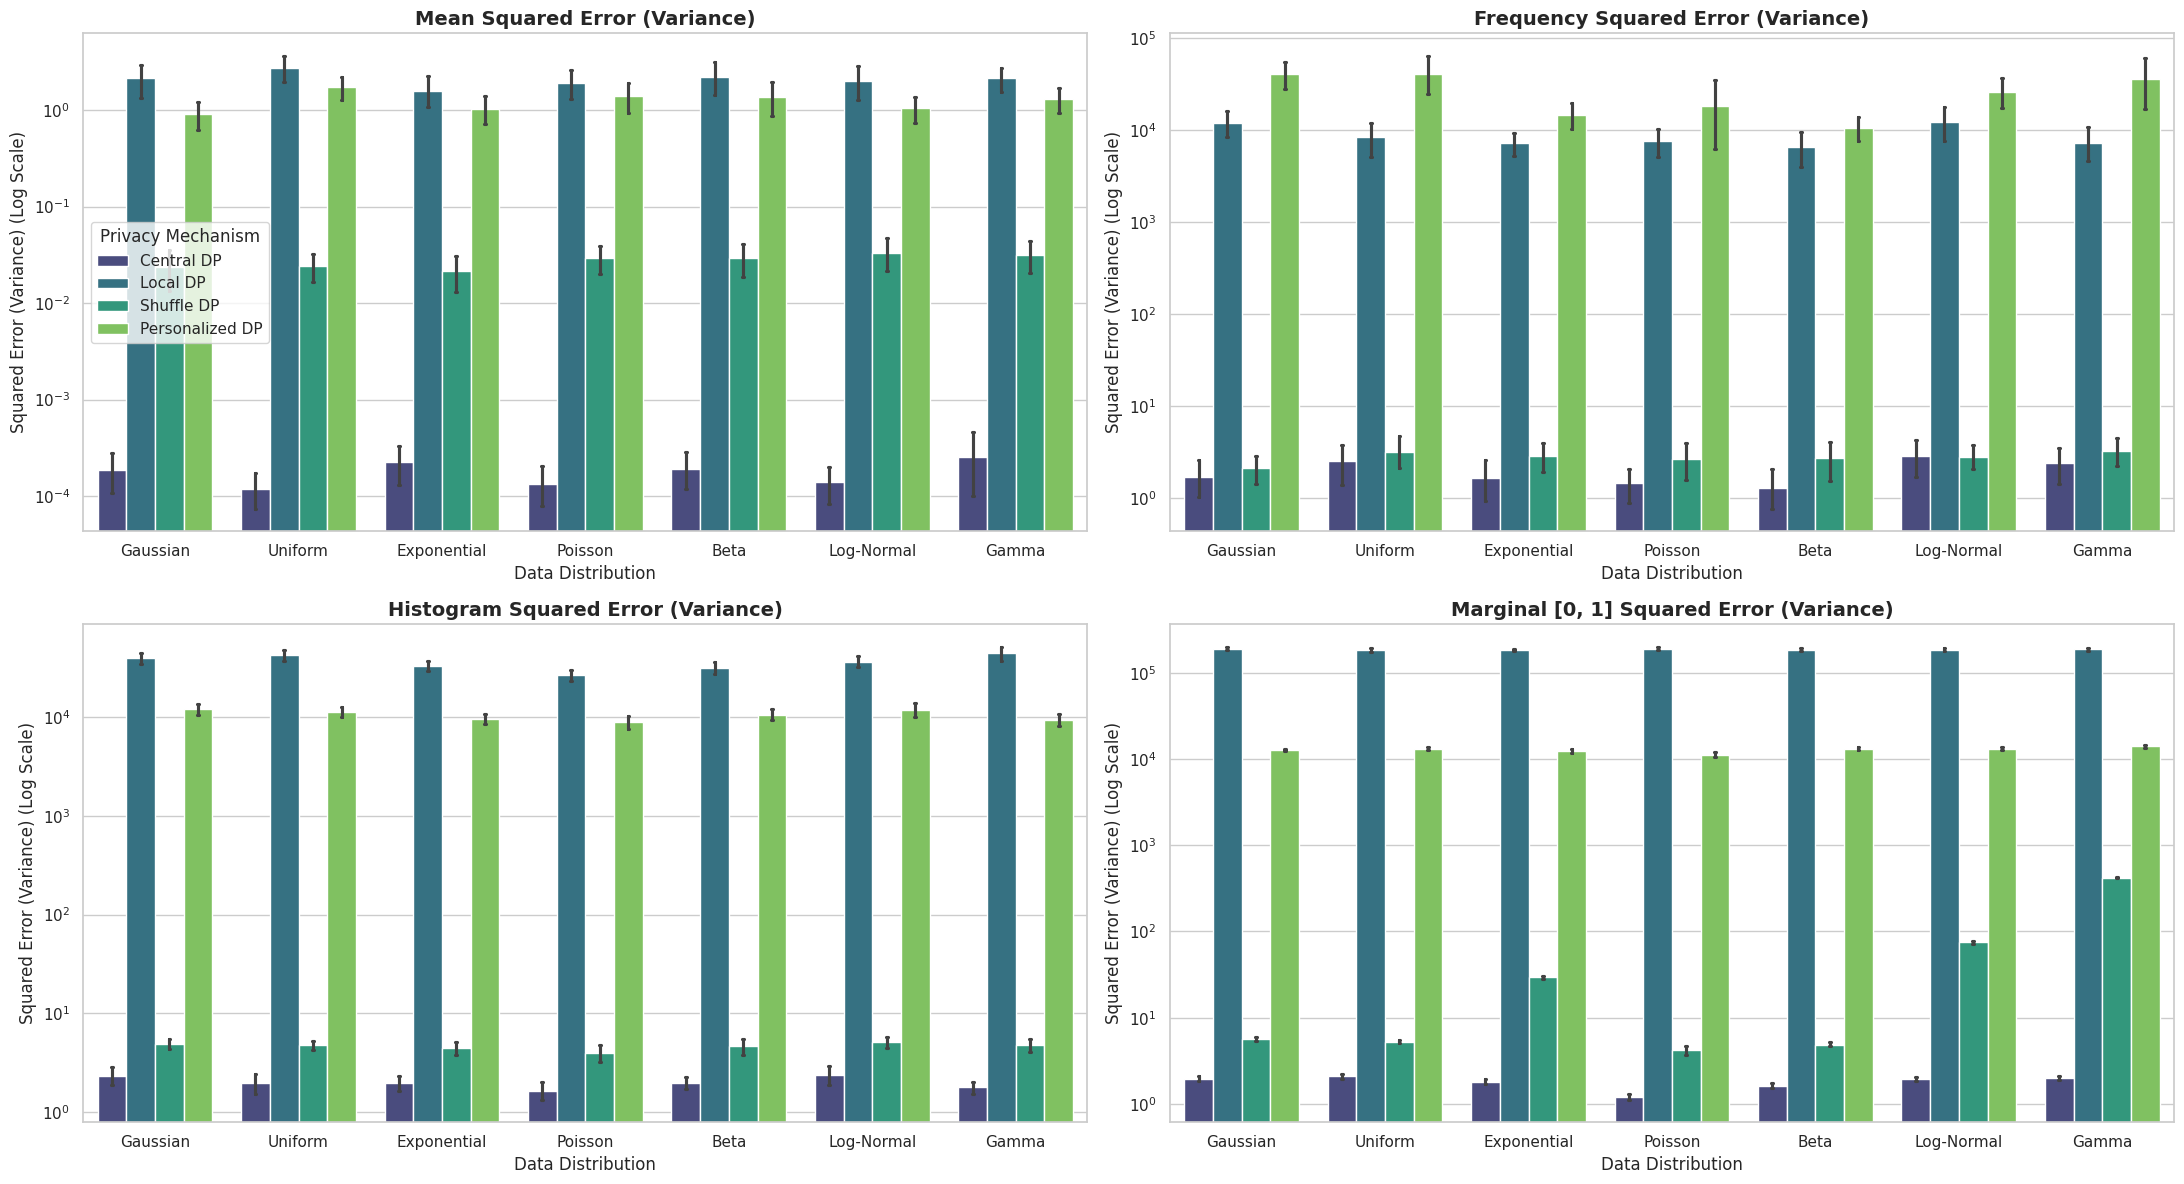
\includegraphics[width=0.48\textwidth]{figs/mse.png}
%     \caption{\rl{نمودارهای لگاریتمی میانگین خطای مطلق (\lr{MAE}) و خطای میانگین مربعات (\lr{MSE}) برای ارزیابی واریانس نویز در مدل‌های مختلف.}}
%     \label{fig:res_charts_bar}
% \end{figure}

% برای غلبه بر این چالش بنیادین، مدل محرمانگی مخلوط‌شده (\lr{SDP}) از طریق پدیده‌ی تقویت محرمانگی با هم‌زدن پیام‌ها، توانسته است شکاف عظیم میان نرخ همگرایی $\mathcal{O}\left( \frac{1}{n \al^2} \right)$ و $\mathcal{O}\left( \frac{1}{n^2 \eps^2} \right)$ را تا حد زیادی پر کند (همان‌طور که در نمودارهای لگاریتمی شکل \ref{fig:res_charts_bar} مشهود است). با بهره‌گیری از یک مخلوط‌کننده ایمن، خطای \lr{MSE} تخمین میانگین در این مدل برای توزیع گوسی به $0.0236$ و برای توزیع نمایی به $0.0215$ کاهش یافته است که نشان‌دهنده‌ی بازیابی خیره‌کننده‌ی ظرفیت کانال اطلاعاتی است. در کنار آن، مدل شخصی‌سازی‌شده (\lr{PDP}) با اتخاذ میانگین‌گیری وزن‌دار، عملکردی میانی ارائه می‌دهد که منجر به کاهش خطای \lr{MSE} گوسی به مقدار $0.9041$ شده است؛ هرچند به دقت مدل مخلوط‌شده نمی‌رسد، اما تأثیر مخرب حساسیت‌های بالای امنیتی را مهار می‌کند.

% \begin{figure}[htbp]
%     \centering
%     \includegraphics[width=1\textwidth]{image_0d90b0.jpg}
%     \caption{\rl{اعتبارسنجی مدل‌های \lr{DP} در برابر کران‌های پایین مینی‌مکس نظری. نمودارها رفتار مجانبی خطای \lr{MSE} را نسبت به اندازه‌ی نمونه ($N$) در مقادیر مختلف بودجه محرمانگی نشان می‌دهند.}}
%     \label{fig:res_minimax_validation}
% \end{figure}

% برای درک عمیق‌تر این شکاف کارایی و تأیید ماهیت اطلاعاتی آن، رفتار مجانبی خطا نسبت به اندازه‌ی فضای نمونه ($n$) را تحت سطوح مختلف بودجه محرمانگی مورد ارزیابی قرار دادیم (شکل \ref{fig:res_minimax_validation}). در نمودارهای لگاریتمی رسم‌شده، شیب منحنی‌ها نشان‌دهنده‌ی نرخ همگرایی مدل‌هاست. همان‌طور که مشاهده می‌شود، داده‌های تجربی مدل موضعی (منحنی قرمز رنگ) با دقتی خیره‌کننده بر کران‌های نظری استخراج‌شده توسط دوچی و همکاران منطبق هستند و دقیقاً از نرخ $\mathcal{O}\left( \frac{1}{n \al^2} \right)$ پیروی می‌کنند \cite{Duchi2013}. هم‌چنین، خطای عملی این مکانیزم‌ها همواره توسط کران‌های مبتنی بر انقباض $f$-واگرایی‌ها که در چارچوب نظری آسوده و همکاران توسعه یافته‌اند (منحنی نقطه‌چین نارنجی)، از بالا محدود شده است \cite{Asoodeh2024}. این تطابق تجربی و نظری تأیید می‌کند که افت دقت در مدل \lr{LDP} یک ضعف الگوریتمی نیست، بلکه یک مانع اطلاعاتی و بنیادین است.

% \textbf{تفسیر شهودی:} این شبیه‌سازی تجربی جامع، ماهیت هندسی محرمانگی را در دنیای واقعی به تصویر می‌کشد. تطابق دقیق منحنی‌های تجربی \lr{LDP} با کران‌های نظری مینی‌مکس (دوچی و آسوده) تأیید می‌کند که مکانیزم‌های موضعی نظیر پاسخ تصادفی، به عنوان عملگرهای انقباضی، اطلاعات فیشر را با ضریب $\al^2$ فشرده می‌سازند. این هزینه عدم اعتماد به این معناست که در سناریوهایی با بودجه‌های محرمانگی سخت‌گیرانه (نظیر $\al \le 1.0$)، خطای ناشی از واریانس نویز به قدری بر سیگنال واقعی غلبه می‌کند که استنتاج در فضاهای با ابعاد بالا عملاً بی‌معنی می‌شود، مگر آنکه از مدل‌های تقویتی نظیر مدل مخلوط‌شده بهره جست که موفق می‌شوند با شکستن پیوند هویتی داده‌ها، ظرفیت کانال اطلاعاتی را تا حد چشمگیری بازیابی کنند.